% Provenance (never printed): see sources/outline_sources.md (Year 3:
% Darcy's law; permeability; aquifer types; the groundwater-flow equation;
% pumping tests; solute transport, in principle).
% Brief: sources/book5/BRIEFS.md, ch. 23. Curves from figdata/bachelor-3/
% theis.py, flow_net.py and advection_dispersion.py; the site of 瓦尔登-3 from
% figdata/shared/region.py (read only). Exercise and problem values in the
% Book 5 scratch calculator calc/ch23.py. The wells, the dam, the tests and
% the solutes are invented.
\chapter{水文地质学}\label{ch:b3:hydrogeology}

一口新井每天从一层石灰岩中抽取 \qty{2160}{m^3} 的水，
该石灰岩位于农场地下几百米处。农场自家水井起初毫无变化。
一个月后，农场水井的水位下降了近 \qty{2}{m}，尽管它
距新井一千米，而抽水站从未从中抽过一滴水。
新井周围的水位并非均匀下降，而是陷成了一个
锥形，并迅速扩展穿过一层岩石，该岩石中的水
本身每天仅移动几厘米。本章建立物理理论，
用以预测两个数字：压力的快速扩散与水的缓慢迁移，
二者均由 1856 年发现的一条经验定律导出。
% ledger: heath:darcy

\begin{recall}
孔隙度、渗透率、地下水位、地下水、含水层、泉
与水井均见于中学教材，水的停留时间与
化石地下水亦然。动力黏度、管中流动的泊肃叶定律
与扩散方程见于物理教材。误差函数
及用它表示的扩散方程的解，见于
第~\ref{ch:b3:lithosphere-thermal-models}~章。瓦尔登丘陵，本系列的虚构地区，
其砂岩、石灰岩、页岩与白垩，
自中学教材起即为练习所用地区。
\end{recall}

\section{水头与达西定律}\label{sec:b3:hydrogeology:darcy}

地下水从单位重量机械能高的地方
流向低的地方。因水流动缓慢，其动能
可忽略不计，该能量由两部分组成：水的高度与
水的压强。

\begin{definition}[水头；水力梯度]\label{def:b3:hydrogeology:head}
饱和地层中某点的\emph{水头}\index{水头}
由下式给出：
\[
h = z + \frac{p}{\rho g} ,
\]
即该点高出基准面的\emph{位置水头} $z$ 与
\emph{压力水头} $p/(\rho g)$ 之和，$p$ 为水高出
大气压强的部分。它是水在一根仅在该点开口的
测压管中上升到的高度。\emph{水力梯度}\index{水力梯度}
为 $\nabla h$；其大小为沿流动方向相距 $L$ 的两点间的
$\Delta h/L$。
\end{definition}

\begin{omfigure}
\centering
\begin{tikzpicture}[>=stealth, font=\small, x=1cm, y=1cm]
\fill[omLithAlluv!60] (0,-0.6) rectangle (7,3.2);
\fill[omSea!45] (0,-0.6) rectangle (7,1.9);
\draw[thick, brown!60!black] (0,3.2) -- (7,3.2);
\draw[omDef, dashed] (0,1.9) -- (7,1.9);
\node[omDef, font=\scriptsize, anchor=south east] at (6.9,1.92) {地下水位};
% piezometer
\fill[white] (3.3,0.4) rectangle (3.7,4.0);
\draw[thick] (3.3,0.7) -- (3.3,4.0); \draw[thick] (3.7,0.7) -- (3.7,4.0);
\draw[thick, densely dotted] (3.3,0.4) -- (3.3,0.7); \draw[thick, densely dotted] (3.7,0.4) -- (3.7,0.7);
\fill[omSea!70] (3.32,0.4) rectangle (3.68,2.6);
\draw[omDef, thick] (3.3,2.6) -- (3.7,2.6);
\fill (3.5,0.55) circle (0.06);
\node[font=\scriptsize, anchor=west] at (3.75,0.55) {滤管，位于点 $P$};
% datum
\draw[black!60] (0,-0.6) -- (7,-0.6);
\node[font=\scriptsize, anchor=north west] at (0,-0.62) {基准面，$z = 0$};
% heads, on the left of the tube
\draw[<->] (2.5,-0.6) -- node[left, font=\scriptsize] {$z$} (2.5,0.55);
\draw[<->] (2.5,0.55) -- node[left, font=\scriptsize] {$p/\rho g$} (2.5,2.6);
\draw[black!40, densely dashed] (2.4,0.55) -- (3.3,0.55);
\draw[black!40, densely dashed] (1.0,2.6) -- (3.3,2.6);
\draw[<->, thick, omThm] (1.1,-0.6) -- node[left, font=\scriptsize] {$h$} (1.1,2.6);
\node[font=\scriptsize, anchor=south] at (3.5,4.0) {测压管};
\end{tikzpicture}

\par\smallskip{\small 测压管，即仅在滤管处开口的一根管。
管中水位即点 $P$ 的\omterm{def:b3:hydrogeology:head}{水头}，即其位置高度
$z$ 与压力\omterm{def:b3:hydrogeology:head}{水头}之和。此处管中水位高于地下水位，
此情形与水向泉或
河流上涌处相同。}\label{fig:b3:hydrogeology:head}
\end{omfigure}

1856 年，法国工程师亨利·达西测量了水流经
砂柱，并发现流量与单位长度上的\omterm{def:b3:hydrogeology:head}{水头}损失成正比。
流动为层流：水沿互不相交的流线流动。
% ledger: heath:darcy

\begin{theorem}[达西定律]\label{thm:b3:hydrogeology:darcy}
在饱和多孔介质中，单位时间内穿过单位面积的
水的体积为
\[
\vec q = -K\,\nabla h ,
\]
其中 $K$ 取决于介质与流体。若介质中的孔隙为
平行直管，半径为 $a$，所占体积之比为 $n$，
则由泊肃叶定律得到本定律，其中
\[
K = \frac{k\rho g}{\mu}, \qquad k = \frac{na^2}{8} ,
\]
$\mu$ 为水的动力黏度。
\end{theorem}
\index{达西定律}

\begin{proof}
第一条陈述即达西的经验定律。沿流向、半径为 $a$ 的管中，
泊肃叶定律给出平均速度 $\bar u =
-(a^2/8\mu)\,\mathrm d(p + \rho gz)/\mathrm dl = -(a^2\rho g/8\mu)\,\mathrm
dh/\mathrm dl$，由于 $p + \rho gz = \rho g h$。管占据任一截面的
比例 $n$，因此单位总面积上的体积为
$q = n\bar u = -(na^2/8)(\rho g/\mu)\,\mathrm dh/\mathrm dl$.
\end{proof}

真实的孔隙并非笔直的管道；定理给出了该定律的形式
以及它如何随尺度变化。流量与梯度成正比，与孔隙尺寸的平方成正比，
并与黏度成反比：同一种砂
在水温较高时让水通过得更快。

\begin{definition}[比流量；水力传导系数；固有渗透率]\label{def:b3:hydrogeology:darcy}
\emph{比流量}\index{比流量}$\vec q$ 是单位时间内
穿过介质单位面积的水体积（颗粒与孔隙一并计入）。
其中\emph{水力传导系数}\index{水力传导系数}
$K$ 是\omterm{thm:b3:hydrogeology:darcy}{达西定律}的系数，
单位为 \unit{m/s} 或 \unit{m/d}。
介质的\emph{固有渗透率}\index{固有渗透率}为 $k =
K\mu/(\rho g)$，单位为 \unit{m^2}，仅取决于介质本身。
\end{definition}

岩石的\omterm{def:b3:hydrogeology:darcy}{水力传导系数}跨越十二个
数量级，这在物理量中少有。据该领域一项经典综述的图表，
典型范围（以米每天计）为：黏土
\num{e-7} 至 \num{e-4}；粉土与黄土 \num{e-3} 至 2；粉质砂 0.04 至
10；纯净砂 0.3 至 150；砾石 100 至 4000；页岩 \num{e-8} 至
\num{e-4}；砂岩 \num{e-5} 至 0.4；碳酸盐岩
仅有裂隙时为 \num{e-4}，有洞穴时达数千；火成岩与
变质岩在未裂隙化时低于 \num{e-8}，裂隙化后可达几。
此外，多数岩石沿层理方向的导水性比
垂直层理方向更好。
% ledger: heath:darcy, heath:k-chart

\omterm{def:b3:hydrogeology:darcy}{比流量}是穿过整个面积的通量；水
仅在孔隙中流动，且流速更快。

\begin{definition}[渗流速度]\label{def:b3:hydrogeology:seepage}
\emph{渗流速度}\index{渗流速度}是 $\vec v = \vec
q/n_e$，即孔隙中水的平均速度，其中 $n_e$ 为
有效孔隙度，即水流经的连通孔隙所占
的比例。
\end{definition}

一种粗砂，$K = \qty{60}{m/d}$，梯度为千分之一，孔隙度为 0.20，水的流速为 \qty{0.3}{m/d}；一种黏土，$K =
\qty{e-4}{m/d}$，梯度为十分之一，孔隙度为 0.50，其流速为
\qty{2e-5}{m/d}，每年不足一厘米。地下水通常不在地下河中
流动，石灰岩中的洞穴与熔岩中的管道除外。
以上均为平均值：污染物运移时，
其最快的部分可能
快数倍。
% ledger: heath:velocity

\section{含水层}\label{sec:b3:hydrogeology:aquifers}

\begin{definition}[承压含水层与潜水含水层；弱透水层]\label{def:b3:hydrogeology:aquifer-types}
\emph{潜水含水层}\index{潜水含水层}是指上界面为
地下水位的含水层。
\emph{承压含水层}\index{承压含水层}是指上覆一层
传导率低得多的岩层，因而其中的水处于承压状态：在
打到该层的井中，水位升至含水层顶部之上，到达其
测压水面。能减缓但不能阻断含水层之间水流通过的
低传导率岩层，称为
\emph{弱透水层}\index{弱透水层}。
\end{definition}

\begin{definition}[导水系数；储水系数；给水度]\label{def:b3:hydrogeology:storage}
含水层的\emph{导水系数}\index{导水系数}，若其厚度为
$b$，则其值为 $T = Kb$，即单位梯度下单位宽度的流量，单位为
\unit{m^2/d}。其\emph{储水系数}\index{储水系数}（亦称储存系数）$S$ 是
\omterm{def:b3:hydrogeology:head}{水头}下降一个单位时，单位面积含水层释放的水体积，
其为无量纲的。
岩石的\emph{给水度}\index{给水度}$S_y$ 为
地下水位下降穿过该岩石时，单位体积岩石
依靠重力排出的水体积。
\end{definition}

两类含水层释放水的方式不同。\omterm{def:b3:hydrogeology:aquifer-types}{承压含水层}中，
\omterm{def:b3:hydrogeology:head}{水头}下降而孔隙仍保持充满：水略有膨胀，
且含水层承受上覆岩石更多的重量，因而
略有压缩。仅水的膨胀所释放的量约为
\num{9e-7} 立方米（每立方米含水层、每米\omterm{def:b3:hydrogeology:head}{水头}）；
加上压缩的作用，多数\omterm{def:b3:hydrogeology:aquifer-types}{承压含水层}的\omterm{def:b3:hydrogeology:storage}{储水系数}为
\num{e-5} 至 \num{e-3}。在\omterm{def:b3:hydrogeology:aquifer-types}{潜水含水层}中，地下水位下降，
其上方孔隙排水：\omterm{def:b3:hydrogeology:storage}{储水系数}即\omterm{def:b3:hydrogeology:storage}{给水度}，约为 0.1
至 0.3，比前者大一百至一万倍。使用中的含水层的\omterm{def:b3:hydrogeology:storage}{导水系数}
范围自裂隙岩中的不足 \qty{1}{m^2/d}，直至
洞穴石灰岩与熔岩流中的 \qty{100000}{m^2/d}。当\omterm{def:b3:hydrogeology:aquifer-types}{承压含水层}的
\omterm{def:b3:hydrogeology:head}{水头}长期被抽降时，其内及周围的黏土排水压实，
上方地面随之下沉。
% ledger: heath:storage, heath:transmissivity

\begin{omfigure}
\centering
\begin{tikzpicture}[>=stealth, font=\small, x=1cm, y=1.1cm]
\begin{scope}
\clip (0,-1.3) -- (0,2.0) -- (3.5,2.9) -- (5,3.5) -- (7.5,4.2) -- (11,3.8) -- (11,-1.3) -- cycle;
\fill[lith sandstone] (0,-1.3) rectangle (11,4.5);
\fill[lith limestone] (0,1.8) -- (11,-0.95) -- (11,0.05) -- (0,2.8) -- cycle;
\fill[lith shale] (0,2.8) -- (11,0.05) -- (11,1.25) -- (0,4.0) -- cycle;
\fill[omLithLime!25] (0,4.0) -- (11,1.25) -- (11,4.5) -- (0,4.5) -- cycle;
\end{scope}
\draw[thick, brown!60!black] (0,2.0) -- (3.5,2.9) -- (5,3.5) -- (7.5,4.2) -- (11,3.8);
% water table in the chalk
\draw[omDef, dashed, thick] (4.5,3.0) .. controls (6,3.35) and (8.5,3.35) .. (11,2.8);
\node[omDef, font=\scriptsize, anchor=south] at (6.6,3.32) {地下水位};
% potentiometric surface of the limestone
\draw[omThm, densely dashdotted, thick] (1.4,2.36) -- (11,2.2);
\node[omThm, font=\scriptsize, anchor=south east, fill=white, inner sep=1pt] at (10.9,2.25) {石灰岩的测压水面};
% well 瓦尔登-3
\draw[thick] (2.9,2.74) -- (2.9,1.05); \draw[thick] (3.1,2.8) -- (3.1,1.05);
\fill[omDef!35] (2.92,1.05) rectangle (3.08,2.33);
\draw[omThm, thick] (2.85,2.33) -- (3.15,2.33);
\node[font=\scriptsize, anchor=south] at (3.0,2.95) {瓦尔登-3};
% labels
\node[font=\scriptsize, fill=white, inner sep=1pt] at (7.5,0.45) {石灰岩：承压含水层};
\node[font=\scriptsize, fill=white, inner sep=1pt] at (7.5,1.5) {页岩：隔水层};
\node[font=\scriptsize, fill=white, inner sep=1pt] at (8.4,2.8) {白垩：潜水含水层};
\node[font=\scriptsize, fill=white, inner sep=1pt] at (7.5,-0.8) {砂岩};
\node[font=\scriptsize, fill=white, inner sep=1pt, align=center] at (0.8,1.75) {石灰岩 \\露头};
\draw[->, omDef, thick] (0.8,3.0) -- (0.8,2.3);
\node[omDef, font=\scriptsize, anchor=south] at (0.8,3.0) {补给};
\end{tikzpicture}

\par\smallskip{\small 瓦尔登丘陵覆盖层的示意剖面，
自西向东，未按比例绘制。白垩层中含有\omterm{def:b3:hydrogeology:aquifer-types}{潜水含水层}，
位于其地下水位以下。侏罗纪石灰岩在
露头处获得补给，并承压于页岩之下：习题中的瓦尔登-3 井
穿过页岩钻成，仅与石灰岩相通，其水位
上升至测压面，远高于含水层的
顶部，但仍低于地面。}\label{fig:b3:hydrogeology:aquifers}
\end{omfigure}
% ledger: region:name

\section{地下水流方程}\label{sec:b3:hydrogeology:flow-equation}

\begin{theorem}[地下水流方程]\label{thm:b3:hydrogeology:flow-equation}
在\omterm{def:b3:hydrogeology:storage}{导水系数} $T$ 与\omterm{def:b3:hydrogeology:storage}{储水系数} $S$ 为常数的\omterm{def:b3:hydrogeology:aquifer-types}{承压含水层}中，
水流沿水平方向，\omterm{def:b3:hydrogeology:head}{水头} $h(x, y, t)$ 满足
\[
S\,\frac{\partial h}{\partial t} = T\nabla^2h + W ,
\]
$W$ 为单位面积、单位时间内经补给增加或
经抽水移除（取负值）的水的体积。稳定流动且无源时，$\nabla^2h =
0$。
\end{theorem}
\index{地下水流方程}

\begin{proof}
取含水层中面积为 $\mathrm dx\,\mathrm dy$ 的柱体。单位
宽度贯穿全厚的流量为 $-T\nabla h$，由\omterm{thm:b3:hydrogeology:darcy}{达西定律}乘以
$b$ 得到。净流入量为 $-\nabla\cdot(-T\nabla h)\,\mathrm dx\,\mathrm
dy = T\nabla^2h\,\mathrm dx\,\mathrm dy$。柱体内储存的水量
以速率 $S\,(\partial h/\partial t)\,\mathrm dx\,\mathrm dy$ 变化，
由 $S$ 的定义。质量守恒中，水的密度取为常数，
储存量等于流入量加上源项。
\end{proof}

它即物理课本中的扩散方程，只是以水力
扩散系数 $T/S$ 代替热扩散系数。对承压石灰岩，取
$T = \qty{450}{m^2/d}$，$S = \num{2e-4}$，则扩散系数为
\qty{2.25e6}{m^2/d}：\omterm{def:b3:hydrogeology:head}{水头}变化扩散 \qty{1}{km} 距离
所需时间约 $L^2S/T$，即半天。同一石灰岩若为潜水，取 $S =
0.2$，所需时间将长千倍。压力扩散很快，
而水的运动很慢：即开篇所述的两个数字。

\begin{proposition}[向井的稳定径向流]\label{prop:b3:hydrogeology:thiem}
一口井以流量 $Q$ 从\omterm{def:b3:hydrogeology:storage}{导水系数}为 $T$ 的\omterm{def:b3:hydrogeology:aquifer-types}{承压含水层}中抽水，
流动为稳定径向流。距井两处距离 $r_1 < r_2$ 处的
降深之差为
\[
s_1 - s_2 = \frac{Q}{2\pi T}\ln\frac{r_2}{r_1} .
\]
\end{proposition}

\begin{proof}
过井周围每个半径为 $r$ 的圆，流入量为 $Q = 2\pi r
T\,\mathrm dh/\mathrm dr$。积分 $\mathrm dh = (Q/2\pi T)\,\mathrm
dr/r$，自 $r_1$ 积分至 $r_2$，并记 $s = h_0 - h$，即得结论。
\end{proof}

二维稳定流动可用\omterm{def:b3:hydrogeology:flow-net}{流网}表示。

\begin{definition}[流网]\label{def:b3:hydrogeology:flow-net}
称\emph{流网}\index{流网}为均匀、各向同性剖面中地下水稳定流动的
一种作图，由两族曲线构成：等势线，
即\omterm{def:b3:hydrogeology:head}{水头}相等的线，以及水流所沿的流线。
流线与等势线处处正交，且在流网中
其间距使各网格单元为曲边正方形。
\end{definition}

\begin{method}[由流网求渗流量]\label{met:b3:hydrogeology:flow-net}
\leavevmode
\begin{enumerate}
\item 画出边界：不透水边界为一条流线；水体的
  河床，\omterm{def:b3:hydrogeology:head}{水头}固定处为等势线。
\item 在最高与最低\omterm{def:b3:hydrogeology:head}{水头}之间画 $N_d$ 个\omterm{def:b3:hydrogeology:head}{水头}降，每降 $\Delta h
  = H/N_d$，并反复试画出构成 $N_f$ 个流槽的流线，
  直至每个网格均为曲边正方形。
\item 每个流槽沿垂直于
  剖面方向的单位长度携带 $K\Delta h$，方格的长与宽相消，总流量为 $q =
  KHN_f/N_d$。
\end{enumerate}
\end{method}

\begin{omfigure}
\centering
\begin{tikzpicture}
\begin{axis}[width=0.95\linewidth, height=0.36\linewidth, axis equal image,
  xmin=-60, xmax=60, ymin=-20, ymax=13, xlabel={$x$ (\unit{m})}, ylabel={$z$ (\unit{m})},
  tick label style={font=\scriptsize}, label style={font=\small}, clip=false]
% computed in figdata/bachelor-3/flow_net.py
\fill[omLithAlluv!35] (axis cs:-60,-20) rectangle (axis cs:60,0);
\fill[omSea!40] (axis cs:-60,0) rectangle (axis cs:-10,11.2);
\fill[omSea!40] (axis cs:10,0) rectangle (axis cs:60,1.2);
\fill[black!35] (axis cs:-10,0) -- (axis cs:-10,12.5) -- (axis cs:-5,12.5) -- (axis cs:10,0) -- cycle;
\pgfplotsinvokeforeach{1,...,9}{
  \addplot[omThm, thin, unbounded coords=jump] table[x=x, y=z] {figdata/out/bachelor-3-flow_net-h-#1.dat};}
\pgfplotsinvokeforeach{1,...,4}{
  \addplot[omMeth, thick, unbounded coords=jump] table[x=x, y=z] {figdata/out/bachelor-3-flow_net-psi-#1.dat};}
\draw[very thick] (axis cs:-60,-20) -- (axis cs:60,-20);
\node[font=\scriptsize, anchor=south] at (axis cs:45,-19.6) {不透水岩层};
\node[font=\scriptsize, align=center] at (axis cs:-36,6) {水库，\qty{10}{m} 高出 \\下游水体};
\node[font=\scriptsize, anchor=south] at (axis cs:35,1.4) {下游水体};
\node[font=\scriptsize] at (axis cs:-4,4) {坝};
\end{axis}
\end{tikzpicture}

\par\smallskip{\small 坝下渗流，坝宽 \qty{20}{m}，坐落于
厚 \qty{20}{m} 的砂层之上，水库比
下游水体高 \qty{10}{m}，分别对\omterm{def:b3:hydrogeology:head}{水头}与
流函数求解拉普拉斯方程算得。细线为等势线，每米\omterm{def:b3:hydrogeology:head}{水头}一条。
粗线为四条流线，它们与坝底及底面一起
共围成五个流槽。算得的渗流量为 $0.51\,KH$，每米
坝长；\omterm{def:b3:hydrogeology:flow-net}{流网}给出 $KH \times 5/10 = 0.50\,KH$。}\label{fig:b3:hydrogeology:flow-net}
\end{omfigure}

\section{抽水试验}\label{sec:b3:hydrogeology:pumping}

向井的稳定流动很少见：达到新的稳态可能需要数月或
数年，也可能永远达不到。1935 年，美国地质调查局的泰斯
给出了以恒定速率抽水时，井周降深随时间变化的关系，
由此只需数小时或数天的试验，即可求得
含水层的\omterm{def:b3:hydrogeology:storage}{导水系数}与\omterm{def:b3:hydrogeology:storage}{储水系数}。
% ledger: heath:theis

\begin{theorem}[泰斯解]\label{thm:b3:hydrogeology:theis}
一口完全贯穿的无限、均匀\omterm{def:b3:hydrogeology:aquifer-types}{承压含水层}的井，
\omterm{def:b3:hydrogeology:storage}{导水系数}为 $T$、\omterm{def:b3:hydrogeology:storage}{储水系数}为 $S$，在 $t = 0$ 时开始以
恒定流量 $Q$ 抽水。距井 $r$ 处的降深为
\[
s(r, t) = \frac{Q}{4\pi T}\,W(u), \qquad u = \frac{r^2S}{4Tt}, \qquad
W(u) = \int_u^\infty\frac{\mathrm e^{-y}}{y}\,\mathrm dy = -\gamma - \ln u +
u - \frac{u^2}{2\cdot2!} + \frac{u^3}{3\cdot3!} - \cdots,
\]
其中 $\gamma = \num{0.5772}$。$W$ 称为井函数。
\end{theorem}
\index{泰斯解}

\begin{proof}
径向形式的渗流方程为 $S\,\partial s/\partial t =
T\,r^{-1}\partial_r(r\,\partial_rs)$，边界条件为：$s = 0$（$t = 0$ 时），$s \to 0$（$r \to \infty$ 时），
以及 $2\pi rT\,\partial_rs \to -Q$（$r \to 0$ 时）。
数据中并无单独的长度或时间量，故试取 $s = f(u)$，其中 $u =
r^2S/4Tt$。由 $\partial_ru = 2u/r$ 与 $\partial_tu = -u/t$，得 $r\,\partial_rs =
2uf'$，$r^{-1}\partial_r(r\,\partial_rs) = (4u/r^2)(uf')'$，以及 $\partial_ts =
-(u/t)f'$。将方程乘以 $r^2/(4Tu)$，得 $(uf')' = -uf'$：
令 $g = uf'$，则 $g' = -g$，$g = c\,\mathrm e^{-u}$。由井条件 $2\pi T\cdot2uf' \to -Q$（$u \to 0$）得 $c =
-Q/4\pi T$，又由 $f(\infty) = 0$ 得 $f(u) = (Q/4\pi T)\int_u^\infty
\mathrm e^{-y}y^{-1}\,\mathrm dy$。由
$W(u) = -\gamma - \ln u + \int_0^u(1 - \mathrm e^{-y})\,y^{-1}\,\mathrm dy$ 出发，逐项积分即得级数，
其中常数为欧拉常数。
\end{proof}

\begin{proposition}[库珀–雅各布近似]\label{prop:b3:hydrogeology:cooper-jacob}
当 $u \le 0.05$ 时，泰斯降深近似为
\[
s = \frac{2.3\,Q}{4\pi T}\log_{10}\frac{2.25\,Tt}{r^2S} :
\]
以 $\log_{10}t$ 为横坐标作图时，降深为一条直线，其每对数周期的升高量为 $\Delta s$，
由此可得 $T = 2.3\,Q/(4\pi\Delta s)$，而该直线与 $s = 0$ 的截距位于
$t_0$ 处，由此得 $S = 2.25\,Tt_0/r^2$。
\end{proposition}
\index{库珀–雅各布近似}

\begin{proof}
当 $u$ 很小时，级数为 $W \approx -\gamma - \ln u = \ln(\mathrm
e^{-\gamma}/u) = \ln(0.5615\cdot4Tt/r^2S) = \ln(2.25\,Tt/r^2S)$；下一项
$u$ 至多为 \num{0.05}，在此范围内不超过 $W$ 的 \qty{2}{\percent}。
由 $\ln x = 2.3\log_{10}x$ 可知，时间每增大
十倍，降深升高 $2.3\,Q/4\pi T$，并在 $2.25\,Tt_0 = r^2S$ 时为零。
\end{proof}

\begin{omfigure}
\begin{tikzpicture}
\begin{groupplot}[group style={group size=2 by 1, horizontal sep=1.5cm},
  width=0.48\linewidth, height=0.4\linewidth,
  tick label style={font=\scriptsize}, label style={font=\small}, title style={font=\small}]
\nextgroupplot[xmode=log, xlabel={$1/u$}, ylabel={$W(u)$}, xmin=0.1, xmax=1e4, ymin=0, ymax=9,
  title={井函数},
  legend style={font=\scriptsize, at={(0.03,0.97)}, anchor=north west}]
% computed in figdata/bachelor-3/theis.py
\addplot[omDef, thick] table[x=invu, y=W] {figdata/out/bachelor-3-theis-wu.dat};
\addlegendentry{泰斯 $W(u)$}
\addplot[omThm, densely dashed, thick] table[x=invu, y=Wcj] {figdata/out/bachelor-3-theis-cj.dat};
\addlegendentry{$-\gamma - \ln u$}
\addplot[black!40, densely dotted, forget plot] coordinates {(20,0) (20,9)};
\node[font=\scriptsize, black!60, anchor=west] at (axis cs:24,0.6) {$u = 0.05$};
\nextgroupplot[xmode=log, xlabel={抽水开始后的时间（\unit{min}）}, ylabel={降深（\unit{m}）},
  xmin=0.5, xmax=5000, ymin=0, ymax=3.4, title={瓦尔登-3，$r = \qty{60}{m}$},
  legend style={font=\scriptsize, at={(0.03,0.97)}, anchor=north west}]
\addplot[only marks, mark=*, mark size=1.3pt] table[x=tmin, y=s] {figdata/out/bachelor-3-theis-test.dat};
\addlegendentry{实测}
\addplot[omMeth, thick, domain=0.973:5000, samples=2] {0.87221*log10(x/0.973132)};
\addlegendentry{库珀–雅各布直线}
\addplot[black!40, densely dotted, forget plot] coordinates {(11.5,0) (11.5,3.4)};
\end{groupplot}
\end{tikzpicture}

\par\smallskip{\small 左图为泰斯井函数随 $1/u$ 变化的曲线（横轴取对数坐标）及其直线近似，
二者在 $u <
0.05$ 时重合（点线标出）。右图为本题瓦尔登-3 试验中观测井记录的降深，
该观测井距抽水井 \qty{60}{m}，
并对 \qty{11.5}{min} 之后、满足 $u <
0.05$ 的数据点拟合直线：其斜率给出 $T$，截距给出 $S$。}\label{fig:b3:hydrogeology:theis}
\end{omfigure}
% ledger: heath:theis, heath:jacob

\begin{definition}[降落漏斗]\label{def:b3:hydrogeology:cone}
抽水井的\emph{降落漏斗}\index{降落漏斗}是指
抽水井周围地下水位（或测压面）的下降区域，
其梯度向井方向逐渐变陡；
所有的水都须经由井流出。
\end{definition}

由于降深服从线性方程，多口井的\omterm{def:b3:hydrogeology:cone}{降落漏斗}
可以叠加。\omterm{def:b3:hydrogeology:aquifer-types}{承压含水层}的\omterm{def:b3:hydrogeology:storage}{储水系数}很小，\omterm{def:b3:hydrogeology:cone}{降落漏斗}扩展很快，
相邻井的\omterm{def:b3:hydrogeology:cone}{降落漏斗}很快发生干涉；
而\omterm{def:b3:hydrogeology:aquifer-types}{潜水含水层}须排出孔隙中的水，\omterm{def:b3:hydrogeology:cone}{降落漏斗}扩展较慢。\omterm{def:b3:hydrogeology:cone}{降落漏斗}
仅当其截获了足够的补给，或减少了足够多的
含水层向河流和泉的天然排泄，使之与抽水量相平衡时，
\omterm{def:b3:hydrogeology:cone}{降落漏斗}才停止扩展。大量抽取\omterm{def:b3:hydrogeology:aquifer-types}{承压含水层}的水，影响范围很大：1981 年，
约 \qty{277000}{m^3/d} 的水取自大西洋沿岸平原的白垩纪含水层，
该平原位于弗吉尼亚州和北卡罗来纳州，
使其上叠加形成了多个相互重叠的\omterm{def:b3:hydrogeology:cone}{降落漏斗}。
% ledger: heath:cone

\begin{omfigure}
\begin{tikzpicture}
\begin{groupplot}[group style={group size=2 by 1, horizontal sep=1.5cm},
  width=0.48\linewidth, height=0.4\linewidth, y dir=reverse,
  tick label style={font=\scriptsize}, label style={font=\small}, title style={font=\small}]
\nextgroupplot[xlabel={距井的距离 (\unit{m})}, ylabel={降深 (\unit{m})},
  xmin=0, xmax=3000, ymin=0, ymax=6, title={单井的降落漏斗},
  scaled x ticks=false, xticklabel style={/pgf/number format/1000 sep={}},
  legend style={font=\scriptsize, at={(0.97,0.03)}, anchor=south east}]
% computed in figdata/bachelor-3/theis.py
\addplot[omThm!50, thick] table[x=r, y=s] {figdata/out/bachelor-3-theis-cone-1.dat};
\addlegendentry{1 天}
\addplot[omThm!80, thick] table[x=r, y=s] {figdata/out/bachelor-3-theis-cone-10.dat};
\addlegendentry{10 天}
\addplot[omThm!60!black, thick] table[x=r, y=s] {figdata/out/bachelor-3-theis-cone-100.dat};
\addlegendentry{100 天}
\nextgroupplot[xlabel={$x$ (\unit{m})}, ylabel={降深 (\unit{m})},
  xmin=-1500, xmax=1900, ymin=0, ymax=9, title={两口井，10 天},
  scaled x ticks=false, xticklabel style={/pgf/number format/1000 sep={}},
  legend columns=3, legend style={font=\scriptsize, at={(0.5,0.985)}, anchor=north,
  /tikz/every even column/.append style={column sep=3pt}}]
\addplot[omDef, densely dashed] table[x=x, y=s1] {figdata/out/bachelor-3-theis-interf.dat};
\addlegendentry{井位于 0}
\addplot[omMeth, densely dashed] table[x=x, y=s2] {figdata/out/bachelor-3-theis-interf.dat};
\addlegendentry{井位于 400 米}
\addplot[black, thick] table[x=x, y=stot] {figdata/out/bachelor-3-theis-interf.dat};
\addlegendentry{两井共同作用}
\end{groupplot}
\end{tikzpicture}

\par\smallskip{\small 瓦尔登-3 井的泰斯\omterm{def:b3:hydrogeology:cone}{降落漏斗}（$Q =
\qty{2160}{m^3/d}$，$T = \qty{450}{m^2/d}$，$S = \num{2e-4}$），
降深向下绘制。左图为 1、10 和 100 天后的情形：每隔十倍时间，漏斗深度增加的量相同，
而在无限\omterm{def:b3:hydrogeology:aquifer-types}{承压含水层}中，漏斗宽度无限扩展。
右图为相距 \qty{400}{m} 的两口这样的井在 10 天后的情形：
降深相加，两井中点处降深为 \qty{5.5}{m}，
而单井时仅为 \qty{2.7}{m}。}\label{fig:b3:hydrogeology:cone}
\end{omfigure}
% ledger: heath:cone, heath:storage

\begin{inthefield}[抽水试验]
\begin{minipage}[t]{0.55\linewidth}\vspace{0pt}
抽水试验前，水文地质学家先在井中记录一段时间的水位，
以了解试验将叠加其上的水位变化趋势。
随后，水泵以恒定流量抽水，流量保持稳定，由排水管上的
流量计测量，持续数小时至数天。在每口观测井中，
若条件允许，至少应有三口位于不同距离的观测井，
在固定测量点以下测得水位埋深，并于
精确已知的时刻读取，开始的几分钟内读数较多，之后渐少：可用
带刻度的钢卷尺，或电测水位计，其电极接触水面时闭合电路。
如今，常将潜水式压力传感器悬挂于
井中，并与电子记录仪相连，几乎
连续地记录水位。
\end{minipage}\hfill
\begin{minipage}[t]{0.42\linewidth}\vspace{0pt}
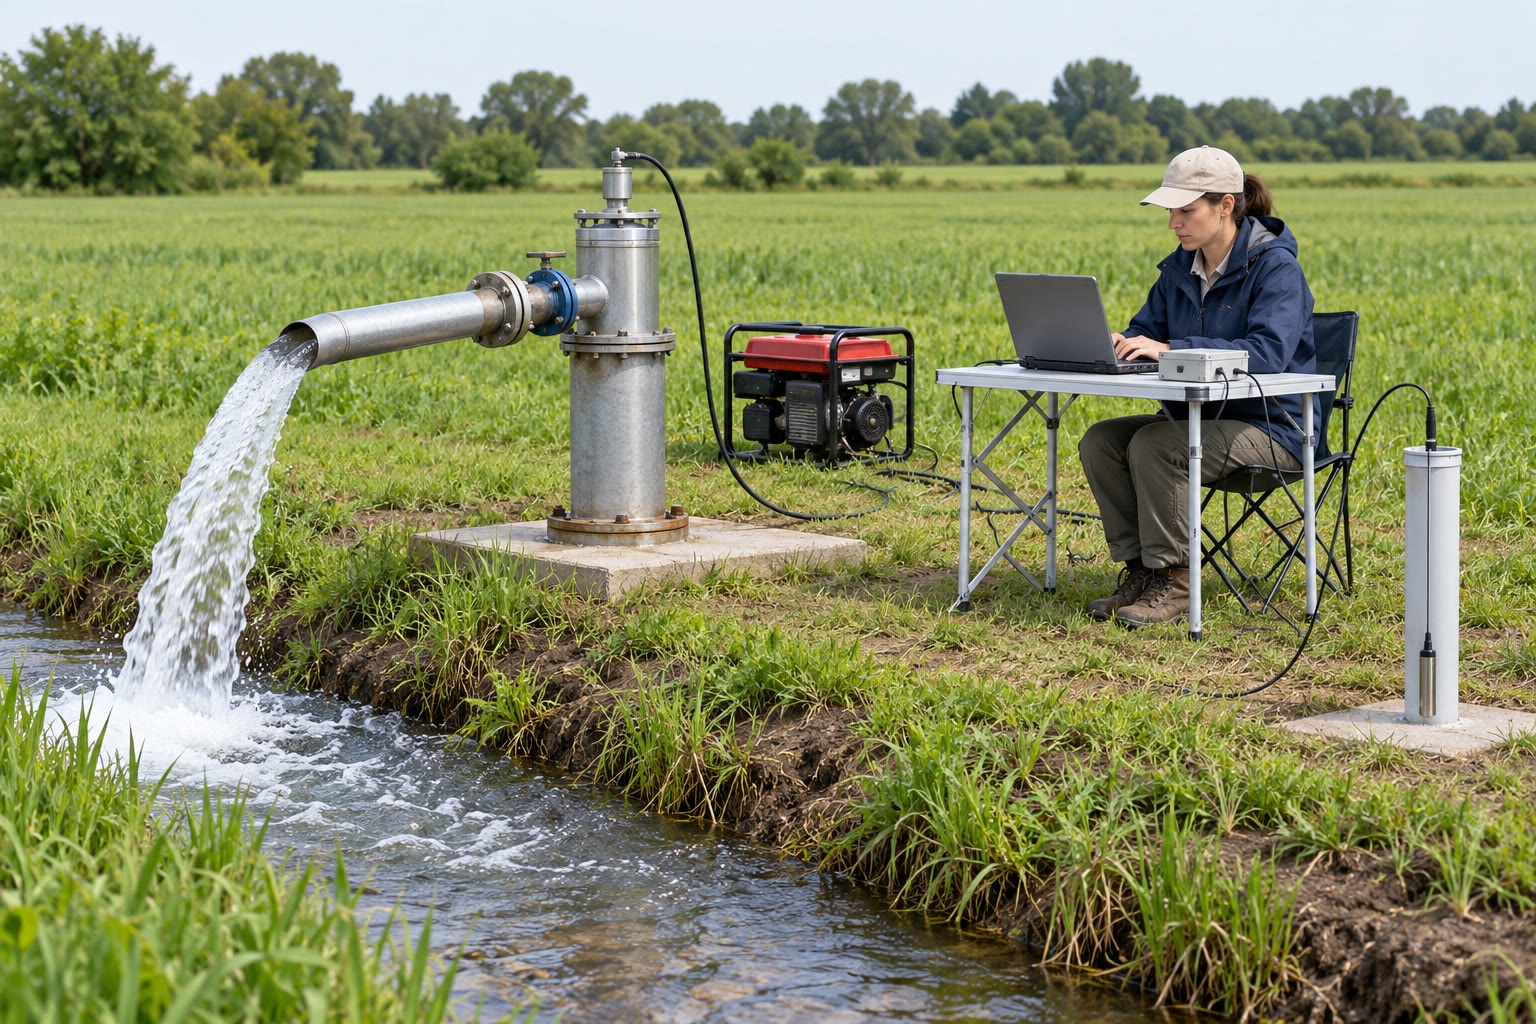
\includegraphics[width=\linewidth]{images/book5/ai/b3-pumping-test.jpg}

{\scriptsize 抽水试验：被抽水井的排水管、
一台发电机，以及记录观测井水位的水文地质学家，
他在笔记本电脑上做记录（AI 生成的插图）。}
\end{minipage}
\end{inthefield}
% ledger: heath:theis, heath:jacob, heath:water-levels, usgs:transducers

\section{溶质运移}\label{sec:b3:hydrogeology:transport}

溶解于地下水中的溶质随水一起以\omterm{def:b3:hydrogeology:seepage}{渗流速度}迁移，
并在迁移中不断扩展：相邻孔隙中的水流速度不同，
路径也各不相同，溶质
同时也发生扩散。

\begin{definition}[水动力弥散；弥散度]\label{def:b3:hydrogeology:ade}
\emph{水动力弥散}\index{水动力弥散}是指溶质在
流动地下水中的扩展，其原因是孔隙间水的流速变化
以及分子扩散。沿流动方向，
其弥散系数为 $D = \alpha_Lv + D^*$，
其中 $v$ 为\omterm{def:b3:hydrogeology:seepage}{渗流速度}，$D^*$ 为有效分子扩散系数，
$\alpha_L$ 为长度量纲的纵向
\emph{弥散度}\index{弥散度}，表征介质的性质。
\end{definition}

\begin{theorem}[对流–弥散方程]\label{thm:b3:hydrogeology:ade}
设沿一维流动方向的\omterm{def:b3:hydrogeology:seepage}{渗流速度} $v$ 为常数，
非反应性溶质的浓度 $C(x, t)$ 满足
\[
\frac{\partial C}{\partial t} = D\,\frac{\partial^2C}{\partial x^2} -
v\,\frac{\partial C}{\partial x} .
\]
若保持浓度 $C_0$ 于 $x = 0$ 处，自 $t = 0$ 起，
在初始不含溶质的介质中，则
\[
\frac{C}{C_0} = \frac12\left[\operatorname{erfc}\frac{x - vt}{2\sqrt{Dt}} +
\mathrm e^{vx/D}\operatorname{erfc}\frac{x + vt}{2\sqrt{Dt}}\right] .
\]
\end{theorem}
\index{对流–弥散方程}

\begin{proof}
取单位截面积、长度为 $\mathrm dx$ 的微元，其有效
孔隙度为 $n_e$，则所储存的溶质量为 $n_eC\,\mathrm dx$，其通量为
$n_e(vC - D\,\partial C/\partial x)$，随水一起迁移，并因弥散而扩展，
与菲克定律所描述的扩散物质的扩散方式一致。由守恒可得
$n_e\partial_tC = -\partial_x[n_e(vC - D\partial_xC)]$，即所求方程。
该公式满足方程及定解条件，在本阶段不加证明地承认；
\cref{exo:b3:hydrogeology:12} 检验其扩展情况。
\end{proof}

在随水一起运动的参考系中，$\xi = x - vt$，方程化为扩散方程，
扩散方程，锋面按 $\sqrt{2Dt} = \sqrt{2\alpha_L
vt} = \sqrt{2\alpha_Lx}$ 扩展：锋面的宽度随
所迁移距离的平方根增长。

\begin{definition}[阻滞因子]\label{def:b3:hydrogeology:retardation}
吸附在颗粒上、处于平衡状态且与浓度成正比的溶质，
其迁移速度慢于水。
其\emph{阻滞因子}\index{阻滞因子（吸附）}为
\[
R = 1 + \frac{\rho_bK_d}{n} ,
\]
其中 $\rho_b$ 为介质的干体积密度，$n$ 为孔隙度，
$K_d$ 为分配系数，即单位质量固体所吸附的质量
与水中浓度之比。溶质的迁移速度为 $v/R$，
并以 $D/R$ 弥散。
\end{definition}

\begin{omfigure}
\begin{tikzpicture}
\begin{groupplot}[group style={group size=2 by 1, horizontal sep=1.5cm},
  width=0.48\linewidth, height=0.4\linewidth,
  tick label style={font=\scriptsize}, label style={font=\small}, title style={font=\small}]
\nextgroupplot[xlabel={时间（天）}, ylabel={距 \qty{100}{m} 处的 $C/C_0$},
  xmin=0, xmax=1000, ymin=0, ymax=1.05, title={穿透曲线},
  legend style={font=\scriptsize, at={(0.97,0.03)}, anchor=south east}]
% computed in figdata/bachelor-3/advection_dispersion.py
\addplot[omDef, thick] table[x=t, y=c1] {figdata/out/bachelor-3-advection_dispersion-btc.dat};
\addlegendentry{$\alpha_L = \qty{1}{m}$}
\addplot[omMeth, thick] table[x=t, y=c3] {figdata/out/bachelor-3-advection_dispersion-btc.dat};
\addlegendentry{$\alpha_L = \qty{3}{m}$}
\addplot[omThm, thick] table[x=t, y=c10] {figdata/out/bachelor-3-advection_dispersion-btc.dat};
\addlegendentry{$\alpha_L = \qty{10}{m}$}
\addplot[black, thick, densely dashed, forget plot] table[x=t, y=cR] {figdata/out/bachelor-3-advection_dispersion-btc.dat};
\node[font=\scriptsize, anchor=west, align=left] at (axis cs:640,0.45) {$\alpha_L = \qty{3}{m}$,\\ $R = 3$};
\addplot[black!40, densely dotted, forget plot] coordinates {(200,0) (200,1.05)};
\nextgroupplot[xlabel={距离（\unit{m}）}, ylabel={150 天后的 $C/C_0$},
  xmin=0, xmax=160, ymin=0, ymax=1.05, title={剖面},
  legend style={font=\scriptsize, at={(0.03,0.03)}, anchor=south west}]
\addplot[omDef, thick] table[x=x, y=c1] {figdata/out/bachelor-3-advection_dispersion-profile.dat};
\addlegendentry{$\alpha_L = \qty{1}{m}$}
\addplot[omMeth, thick] table[x=x, y=c3] {figdata/out/bachelor-3-advection_dispersion-profile.dat};
\addlegendentry{$\alpha_L = \qty{3}{m}$}
\addplot[omThm, thick] table[x=x, y=c10] {figdata/out/bachelor-3-advection_dispersion-profile.dat};
\addlegendentry{$\alpha_L = \qty{10}{m}$}
\addplot[black!40, densely dotted, forget plot] coordinates {(75,0) (75,1.05)};
\end{groupplot}
\end{tikzpicture}

\par\smallskip{\small 溶质在 $x = 0$ 处连续注入
\omterm{def:b3:hydrogeology:seepage}{渗流速度}为 \qty{0.5}{m/d} 的水流中。左图为
顺流方向 \qty{100}{m} 处的浓度随时间的变化：水本身于
200 天后到达（虚线）；\omterm{def:b3:hydrogeology:ade}{弥散度}越大，最先出现的示踪剂越早，
而完全浓度出现得越晚。被吸附的溶质 $R =
3$，到达时间延后为三倍。右图为 150 天后
沿流动方向的浓度分布，此时水已迁移 \qty{75}{m}
（虚线）。}\label{fig:b3:hydrogeology:transport}
\end{omfigure}

\omterm{def:b3:hydrogeology:ade}{弥散度}很难测量，实践中常
依经验法则来确定。最古老的一条规则取纵向\omterm{def:b3:hydrogeology:ade}{弥散度}为
污染羽长度的十分之一。一项于
1992 年发表的现场测量汇编表明：\omterm{def:b3:hydrogeology:ade}{弥散度}随实验尺度增大而增大，
大尺度上可靠的数值很少，而在任一尺度上，
数值的分布范围可跨越两到三个数量级。
% ledger: epa:dispersivity

\section{练习}

\begin{exercise}[$\star$]\label{exo:b3:hydrogeology:1}
两支测压管并排设置在高出
基准面 \qty{120.0}{m} 的地面上。第一支的滤水管位于 \qty{40}{m} 深处，其水位
位于地面以下 \qty{12.5}{m}；第二支的滤水管位于 \qty{80}{m} 深处，
其水位位于地面以下 \qty{15.0}{m}。计算两个滤水管处的位置
\omterm{def:b3:hydrogeology:head}{水头}、压力\omterm{def:b3:hydrogeology:head}{水头}和\omterm{def:b3:hydrogeology:head}{水头}。两个滤水管之间的水流方向如何，
并在怎样的竖直方向梯度下流动？
\end{exercise}

\begin{exercise}[$\star$]\label{exo:b3:hydrogeology:2}
一根长 \qty{50}{cm}、直径 \qty{10}{cm} 的砂柱，$K =
\qty{12}{m/d}$，有效孔隙度为 0.35，水流在
\qty{30}{cm} 的\omterm{def:b3:hydrogeology:head}{水头}差作用下流过。计算\omterm{def:b3:hydrogeology:darcy}{比流量}、
每小时流量（以升计）和\omterm{def:b3:hydrogeology:seepage}{渗流速度}。
\end{exercise}

\begin{exercise}[$\star$]\label{exo:b3:hydrogeology:3}
某石灰岩对 \qty{10}{\celsius} 水的 $K = \qty{2.5}{m/d}$，
（$\rho = \qty{999.7}{kg/m^3}$，$\mu = \qty{1.306e-3}{Pa.s}$）。计算其
\omterm{def:b3:hydrogeology:darcy}{固有渗透率}，以及其对
\qty{20}{\celsius} 水的\omterm{def:b3:hydrogeology:darcy}{水力传导系数}（$\rho = \qty{998.2}{kg/m^3}$，$\mu =
\qty{1.002e-3}{Pa.s}$）。
\end{exercise}
% ledger: nist:water

\begin{exercise}[$\star$]\label{exo:b3:hydrogeology:4}
瓦尔登-3 处承压石灰岩的厚度为 \qty{180}{m}，$K =
\qty{2.5}{m/d}$。计算其\omterm{def:b3:hydrogeology:storage}{导水系数}，以及若仅考虑水的膨胀，
每米含水层、每米\omterm{def:b3:hydrogeology:head}{水头}释放 \num{9e-7} 的水量时所对应的\omterm{def:b3:hydrogeology:storage}{储水系数}，
并与 $S = \num{2e-4}$ 进行比较。
\end{exercise}
% ledger: heath:storage

\begin{exercise}[$\star\star$]\label{exo:b3:hydrogeology:5}
以 \qty{1500}{m^3/d} 的速率长时间抽水后，降深已
稳定不变：在距抽水井 \qty{20}{m} 的观测井中降深为 \qty{2.35}{m}，
另一口距其 \qty{200}{m} 的观测井中降深为 \qty{0.82}{m}。该含水层为
\omterm{def:b3:hydrogeology:aquifer-types}{承压含水层}，厚 \qty{40}{m}。计算其\omterm{def:b3:hydrogeology:storage}{导水系数}和
\omterm{def:b3:hydrogeology:darcy}{水力传导系数}。
\end{exercise}

\begin{exercise}[$\star\star$]\label{exo:b3:hydrogeology:6}
一口井以 \qty{1200}{m^3/d} 的速率从\omterm{def:b3:hydrogeology:aquifer-types}{承压含水层}抽水，含水层的 $T =
\qty{300}{m^2/d}$，$S = \num{5e-4}$。计算 $u$、$W(u)$（由
级数求得）以及距井 \qty{300}{m} 处在 1 天后和 10 天后的降深。
\end{exercise}

\begin{exercise}[$\star\star$]\label{exo:b3:hydrogeology:7}
对瓦尔登-3 井的试验（$T = \qty{450}{m^2/d}$，$S = \num{2e-4}$），经过多少分钟后，
距抽水井 \qty{60}{m} 和 \qty{500}{m} 的观测井中，可以使用库珀–雅各布直线？
这说明短时间试验的观测井
应布置在何处？
\end{exercise}

\begin{exercise}[$\star\star$]\label{exo:b3:hydrogeology:8}
瓦尔登石灰岩中相距 \qty{400}{m} 的两口井，每口井各以 \qty{2160}{m^3/d} 抽水。
计算 10 天后两井中点处的降深，
以及仅由第一口井引起的、第二口井所在处的降深。为什么每口井的
抽水都会使另一口井多花钱？
\end{exercise}

\begin{exercise}[$\star\star$]\label{exo:b3:hydrogeology:9}
在坝下的\omterm{def:b3:hydrogeology:flow-net}{流网}中，数出流道数和\omterm{def:b3:hydrogeology:head}{水头}降落数。
已知 $K = \qty{5}{m/d}$ 和 $H = \qty{10}{m}$，计算每米坝长的
渗流量，以及坝长 \qty{300}{m} 时的渗流量。
\end{exercise}

\begin{exercise}[$\star\star\star$]\label{exo:b3:hydrogeology:10}
将干净砂模拟为半径 \qty{50}{\micro\metre}、孔隙度为 0.30 的直管。
计算 $k$ 和 $K$（水温取 \qty{20}{\celsius}，
与\cref{exo:b3:hydrogeology:3}相同），
并与干净砂的取值范围相比较。该模型忽略了真实砂的哪些特征，
以及每一种特征使 $K$ 向哪个方向变化？
\end{exercise}
% ledger: nist:water, heath:k-chart

\begin{exercise}[$\star\star\star$]\label{exo:b3:hydrogeology:11}
(a)~证明库珀–雅各布降深在 $r_0 =
\sqrt{2.25\,Tt/S}$ 处消失。(b)~计算抽水 30 天后，$r_0$ 在
承压瓦尔登石灰岩中的值，以及同一岩层为\omterm{def:b3:hydrogeology:aquifer-types}{潜水含水层}、取 $S =
0.2$ 时的值。(c)~为什么\omterm{def:b3:hydrogeology:aquifer-types}{承压含水层}的\omterm{def:b3:hydrogeology:cone}{降落漏斗}会
到达试验本不打算探测的边界？
\end{exercise}
% ledger: heath:jacob, heath:storage

\begin{exercise}[$\star\star\star$]\label{exo:b3:hydrogeology:12}
(a)~对于较长的迁移距离，$x$ 处的穿透曲线近似为
时间上的正态分布，均值为 $x/v$，标准差为 $\sigma_t
= \sqrt{2\alpha_Lx}/v$。由锋面的展宽 $\sqrt{2Dt}$ 证明这一点。
(b)~在 \qty{100}{m} 处，取 $v = \qty{0.5}{m/d}$，浓度达到 \qty{16}{\percent} 所需的时间
为 \num{152.6}~天，达到 \qty{84}{\percent} 所需的时间为
\num{247.2}~天。估算 $\alpha_L$。(c)~砂质含水层中 $\rho_b =
\qty{1.9}{g/cm^3}$，$n = 0.30$；溶质的 $K_d =
\qty{0.32}{cm^3/g}$。计算 $R$。
\end{exercise}

\section{问题：瓦尔登-3 井的抽水试验}

\begin{problem}[{周末问题——水头、抽水试验与污染物在
瓦尔登丘陵承压石灰岩中的迁移}]
\label{pb:b3:hydrogeology:1}
虚构的瓦尔登-3 井位于瓦尔登丘陵网格上的 (4500, 5000) 处，
地面高程为 \qty{363.2}{m}，自此穿过侏罗纪页岩，进入侏罗纪石灰岩，
石灰岩顶面位于
海拔 \qty{282.5}{m}，底面位于海拔 \qty{102.5}{m}；井在石灰岩的整个厚度上都打开。
试验前，井中的水位位于
地面以下 \qty{45.0}{m}。

\medskip\noindent\textbf{第一部分——含水层及其天然流动。}
\begin{enumerate}
\item 计算该井处页岩与石灰岩的厚度。
\item 计算石灰岩中的\omterm{def:b3:hydrogeology:head}{水头}以及其顶面处的压力\omterm{def:b3:hydrogeology:head}{水头}。
  为什么此处的石灰岩是\omterm{def:b3:hydrogeology:aquifer-types}{承压含水层}？
\item 三个与石灰岩相通的测压管分别位于 P1 (4300, 5250)、P2
  (4850, 5150) 和 P3 (4550, 4650)，其\omterm{def:b3:hydrogeology:head}{水头}分别为 318.96、317.34 和
  \qty{317.52}{m}。设 $h = ax + by + c$，求 $a$ 和 $b$。
\item 计算\omterm{def:b3:hydrogeology:head}{水力梯度}，以及水流所朝方向的
  方位角。
\end{enumerate}

\medskip\noindent\textbf{第二部分——抽水试验。}该井以
\qty{2160}{m^3/d} 的流量抽水两天。在距井 \qty{60}{m} 处的观测井中，
降深如下：
\begin{center}
\begin{tabular}{l*{11}{c}}
\hline
$t$ (\unit{min}) & 1 & 2 & 3 & 5 & 7 & 10 & 15 & 20 & 30 & 45 & 60\\
$s$ (\unit{m}) & 0.18 & 0.36 & 0.48 & 0.64 & 0.77 & 0.88 & 1.04 & 1.15 & 1.30 & 1.45 & 1.56\\
\hline
$t$ (\unit{min}) & 90 & 120 & 180 & 240 & 360 & 480 & 720 & 960 & 1440 & 2160 & 2880\\
$s$ (\unit{m}) & 1.71 & 1.82 & 1.98 & 2.08 & 2.24 & 2.35 & 2.50 & 2.61 & 2.77 & 2.92 & 3.03\\
\hline
\end{tabular}
\end{center}
\begin{enumerate}[resume]
\item 作 $s$ 关于 $\log_{10}t$ 的图。哪些早期数据点偏离了
  直线段，原因是什么？
\item 由直线段部分量出每个对数周期内的降深。
\item 计算\omterm{def:b3:hydrogeology:storage}{导水系数}。
\item 求直线与零降深相交时的时间 $t_0$。
\item 计算\omterm{def:b3:hydrogeology:storage}{储水系数}。
\item 检验所用数据点是否满足 $u \le 0.05$。
\item 计算石灰岩的\omterm{def:b3:hydrogeology:darcy}{水力传导系数}。
\end{enumerate}

\medskip\noindent\textbf{第三部分——\omterm{def:b3:hydrogeology:cone}{降落漏斗}。}此后取 $T =
\qty{450}{m^2/d}$，$S = \num{2e-4}$。
\begin{enumerate}[resume]
\item 计算观测井中 2 天后的泰斯降深，
  并与记录值比较。
\item 距此 \qty{1}{km} 的一口农用井抽取同一石灰岩中的水。计算其
  抽水 30 天后的降深。
\item 计算 30 天后的雅各布距离 $r_0$。这说明
  含水层边缘与瓦尔登断层的什么情况？
\item 计算 30 天内的抽水量。在\omterm{def:b3:hydrogeology:aquifer-types}{承压含水层}中，
  这些水来自何处？
\item 若石灰岩为\omterm{def:b3:hydrogeology:aquifer-types}{潜水含水层}，农用井处的降深与承压情况
  相比将如何？取 $S = 0.18$。
\end{enumerate}

\medskip\noindent\textbf{第四部分——污染物。}溶解态污染物的一处泄漏
点距井 \qty{200}{m}，污染物到达石灰岩中。取
有效孔隙度为 0.18，\omterm{def:b3:hydrogeology:retardation}{阻滞因子}为 2.5。
\begin{enumerate}[resume]
\item 抽水前，计算第一部分中天然流动的\omterm{def:b3:hydrogeology:darcy}{比流量}和
  \omterm{def:b3:hydrogeology:seepage}{渗流速度}。
\item 水流经过 \qty{200}{m} 需要多长时间，污染物
  又需要多长时间？
\item 井在抽水，且泄漏点位于井的上游，流动
  变为指向井的径向流。证明水流到达井所需时间为 $t = \pi n_e b
  r^2/Q$，其中 $r$ 为出发点距井的距离，忽略天然流动，
  并分别对水和污染物计算该时间。
\item 取\omterm{def:b3:hydrogeology:ade}{弥散度}为距离的十分之一这一经验规则，
  估算井处锋面的展宽 $\sqrt{2\alpha_Lx}$。这对
  首次到达意味着什么？
\item 抽水是否应当继续？给出一条支持和一条反对的理由。
\item 给出瓦尔登石灰岩含水层的\omterm{def:b3:hydrogeology:storage}{导水系数}，单位为
  平方米每天，保留两位有效数字。
\end{enumerate}
\end{problem}
% ledger: heath:jacob, heath:theis, heath:storage, epa:dispersivity, region:name
